\documentclass[10pt,conference]{IEEEtran}
\usepackage[T1]{fontenc}
\usepackage{newtxtext,newtxmath,microtype,graphicx,booktabs,tabularx,array,amsmath,url,balance,float,placeins}
\usepackage[hidelinks]{hyperref}
\usepackage{tikz,xcolor}
\definecolor{deepblue}{HTML}{24578B}
\definecolor{paleBlue}{HTML}{E7F0FA}
\definecolor{paleTeal}{HTML}{E4F5F0}
\definecolor{paleAmber}{HTML}{FFF2D8}
\definecolor{paleGray}{HTML}{F2F4F7}
\definecolor{todoRed}{HTML}{B42318}
\usetikzlibrary{arrows.meta,positioning,fit}
\setlength{\tabcolsep}{3pt}
\renewcommand{\arraystretch}{1.10}
\title{From Co-occurring Ambiguities to Action-Ready Robot Tasks: A Study of Structured, Context-Grounded Interpretation}
\author{\IEEEauthorblockN{Mohammed Bangie \hspace{0.5em} (Student No. 2610990)}\IEEEauthorblockA{School of Computer Science and Applied Mathematics\\University of the Witwatersrand, Johannesburg, South Africa\\Supervisors: Steven James and Benjamin Rosman}}
\newcommand{\pending}[1]{\noindent{\color{todoRed}\footnotesize\textbf{TO DO ---} #1}\par}
\newcommand{\todo}[1]{\par\smallskip\noindent{\color{todoRed}\footnotesize\textbf{TO DO ---} #1}\par\smallskip}
\newcommand{\todocell}{\textcolor{todoRed}{\scriptsize\bfseries TBD}}
\begin{document}
\maketitle\thispagestyle{plain}\pagestyle{plain}
\begin{abstract}
A single instruction to a robot may contain several ambiguities at once: an indirect request, an unclear object reference, an imprecise time, or a missing destination. These ambiguities need not prevent action if the surrounding scene and conversation provide enough information to resolve them. This paper plans a text-to-text study using Gemini 2.5 Flash-Lite to recover an intended goal, ground a structured task in input evidence, and request clarification when a critical detail is unresolved. Direct generation and structured interpretation are the principal comparison; independent repeated-model review remains optional. The current evaluation-only release contains 100 cases with author-approved routes and strategy sequences. It does not yet provide complete semantic task references or simulated clarification replies. Primary task-correctness and multi-turn experiments therefore remain pending reference completion and protocol freeze. No numerical performance claims are made.
\end{abstract}
\begin{IEEEkeywords}
Human--robot interaction, language grounding, ambiguity resolution, clarification, task specification, large language models.
\end{IEEEkeywords}
\noindent{\color{todoRed}\footnotesize\textbf{Gemini working source (uncompiled):} This derived planning source updates the preserved original manuscript for the current dataset and Gemini implementation. No revised PDF has been built or visually checked. Red annotations mark pending work. No evaluated predictions or scientific results are reported.}\par\smallskip
\todo{Revise the abstract and Introduction after obtaining verified results; report the actual contribution and principal quantitative finding rather than planned contributions.}
\section{Introduction}
People rarely describe everyday tasks as complete lists of robot actions. A person might say, ``Put the other cup beside the plate on the left, then move it over there.'' The robot must determine which cup and plate are meant, what ``left'' refers to, whether ``it'' denotes the cup or plate, and where the final destination is. Some answers may be present in the scene or earlier conversation; others may require a question. The useful outcome is not a fluent paraphrase but a task description with the right actions, objects, and constraints.

We call a command \emph{co-occurringly ambiguous} when it contains at least two potentially uncertain aspects, such as its intended action, object, location, time, or scope. Co-occurrence does not necessarily mean that the ambiguities depend on each other. For example, identifying a tray may also identify its assigned recipient, whereas choosing a time and choosing a shelf may be independent decisions. The number of ambiguous expressions alone therefore cannot tell us whether the robot should ask for help.

Prior work has studied indirect requests in task-oriented dialogue \cite{mannekote}, classification and clarification of robot commands \cite{clara}, clarification requests during collaborative tasks \cite{codraw}, and mapping vague commands to structured control calls \cite{clarifyvc}. These studies provide important methods, but they do not by themselves establish which combination is necessary to turn instructions with several ambiguity types into fully grounded task specifications. Work on integrating language models into robotic architectures also cautions against evaluating language interpretation only as an isolated fluent output \cite{sarathy}.

Our scope is deliberately limited to \emph{text-to-text interpretation}. The input may describe a physical environment and the robot's available actions, but this study does not perform motion planning or test physical execution. We define an \emph{action-ready task} as a structured description whose required actions, arguments, and constraints are determined from the supplied information or an explicit user clarification. Action readiness does not certify that a real robot can safely execute the task.

This paper sets out three contributions to be evaluated: (i) a goal-first, evidence-grounded task representation that distinguishes resolved details from unresolved ones; (ii) a controlled study of whether this structure and its contextual checks improve over direct Gemini 2.5 Flash-Lite generation; and (iii) an analysis of whether a second Gemini 2.5 Flash-Lite interpretation and optional adjudication justify their additional cost. These are research aims, not claims of demonstrated improvements.

\section{Background and Related Work}
\subsection{Indirect meaning and task interpretation}
A request can communicate an intended action without naming that action directly. Searle distinguishes the literal form of an utterance from an indirect act performed through it \cite{searle1975}, while Grice explains how conversational context supports inferences beyond the words explicitly spoken \cite{grice1975}. These accounts motivate interpreting communicative intent, but do not supply an algorithm for generating action-ready robot tasks. Mannekote \emph{et al.} study the synthetic generation of indirect requests to make task-oriented dialogue data more natural \cite{mannekote}. Zhang \emph{et al.} examine indirect speech in physical human--robot collaboration, where the literal wording and intended collaborative response may differ \cite{tool}. These works establish why interpreting only the surface wording is inadequate. They do not, however, provide a general test of multiple interacting ambiguities within one task specification.

\subsection{Ambiguity and contextual grounding}
AmbiK provides ambiguous task instructions situated in kitchen environments, illustrating how the same instruction can require additional knowledge or clarification \cite{ambik}. VAGUE investigates how visual context can clarify ambiguous expressions \cite{vague}. Context can make one interpretation more plausible than another, but a plausible interpretation still needs evidence.

A useful distinction is between \emph{co-occurrence} and \emph{dependence}. Two ambiguous fields co-occur when both appear in an instruction; they depend on one another when choosing a value for one constrains the possible value of the other. For example, selecting a labelled medicine tray may determine its recipient. In contrast, the tray and an unrelated delivery deadline may each be resolved independently. This distinction affects how ambiguity is evaluated, even when both instructions contain the same number of ambiguity labels.

\subsection{Clarification in human--robot interaction}
CLARA classifies commands using the current situation and supports clarification of ambiguous instructions \cite{clara}. Madureira and Schlangen analyse clarification requests in collaborative CoDraw dialogues, showing that clarification can concern specific missing or uncertain task information \cite{codraw}. An important distinction is that uncertainty about a model prediction does not necessarily mean a required task detail is missing. For the present text-to-text problem, clarification must ultimately be judged by whether it resolves an execution-critical field.

\subsection{Structured task generation and robot capabilities}
ClarifyVC studies the translation of ambiguous vehicle-control commands into structured, schema-aligned calls and uses ambiguity-oriented data augmentation \cite{clarifyvc}. This makes it a close methodological reference, although vehicle functions are more constrained than many general robot tasks. The selected hosted model is Gemini 2.5 Flash-Lite, requested as \texttt{gemini-2.5-flash-lite}; Google documents its thinking support and API configuration \cite{geminimodel,geminithinking}. Direct generation must receive a documented reasoning budget comparable to the structured procedure. Additional prompts alone do not establish a new reasoning capability; live configuration compatibility remains to be verified before evaluation.

\subsection{Research gap}
The literature provides complementary accounts of indirect meaning, grounding, clarification, and structured outputs. The open question addressed here is narrower and testable: for commands containing several ambiguities, does explicitly representing a task's goal, grounded arguments, and unresolved details improve the correctness of the final task compared with direct generation? A related question is whether repeated reasoning with the same model adds value beyond the structured approach. These questions require reference task specifications, not only labels such as ``execute'' and ``clarify.''

\section{Research Questions and Hypotheses}
\textbf{RQ1 (structured interpretation):} Does an explicit, evidence-grounded task representation with action-readiness validation improve complete-task correctness over direct generation with the same hosted model version, input context, and comparable inference budgets?

\emph{H1:} Structured interpretation will increase the proportion of fully correct task specifications and reduce unsupported argument choices relative to direct generation.

\textbf{RQ2 (context and ambiguity dependence):} How do scene descriptions, dialogue history, and explicit checks between task arguments affect correct interpretation, particularly when ambiguities depend on each other?

\emph{H2:} Removing relevant context will reduce grounding accuracy; checking dependencies will be most useful for examples with linked arguments, rather than all multi-ambiguity examples equally.

\textbf{RQ3 (repeated reasoning):} Does an additional independent Gemini 2.5 Flash-Lite interpretation, with optional Gemini 2.5 Flash-Lite adjudication, improve correctness enough to justify extra inference cost?

\emph{H3:} Review may correct some initial interpretations, but its net benefit will be smaller when compared with a structured system given a comparable inference budget. This hypothesis may be rejected if review adds no measurable value.

\section{Methodology}
\subsection{Task and output definition}
The system receives a human instruction $u$, a scene description $s$, previous dialogue $d$, and a natural-language capability description $c$. The current source does not supply a complete machine-readable catalog of permitted action names and required arguments. Such a catalog would need to be separately specified and frozen for fully deterministic capability validation. Its input is
\begin{equation}
 x=(u,s,d,c),\qquad f(x)\in\{T,q\},
 \label{eq:task}
\end{equation}
where $T$ is a structured task and $q$ is a clarification question. The task $T$ contains the intended goal, ordered actions, their arguments, constraints, and evidence for the chosen values. Missing values remain explicitly unresolved rather than being guessed. For the set $R(T)$ of required arguments, we define
\begin{equation}
 \operatorname{Ready}(T)=
 \left[\bigwedge_{a\in R(T)}\operatorname{Grounded}(a,x)\right]
 \land\operatorname{Consistent}(T,c).
 \label{eq:ready}
\end{equation}
Here, $\operatorname{Grounded}(a,x)$ means that the value of argument $a$ is supported by the instruction, scene, dialogue, or an explicit clarification; $\operatorname{Consistent}(T,c)$ means that the task uses valid action arguments and contains no conflicting constraints. These are criteria for a text specification, not a claim of safe or successful physical execution.

\todo{Finalize the strict output schema and automated checks for required actions, grounded arguments, evidence links, and conflicting constraints; distinguish schema validity from semantic correctness.}
\subsection{Co-occurring ambiguity dataset}
We use version 1.0.1 of the \emph{Co-occurring Ambiguity Dataset}, containing 100 source records, all evaluation-only. Historical provenance records 99 from a frozen Pilot-120 subset and one assistant-authored synthetic case; all 100 are included as source inputs in the current release. Each source record supplies an utterance, scene description, dialogue history, and capability description. Author-approved reference routes contain 74 execute and 26 clarify decisions, together with strategy sequences. Native annotation files retain ambiguity labels, capability status, validity, field-status and provenance information. The supplied files do not include complete semantic action/argument specifications, evidence-linked task gold, dependency eligibility labels, or annotated hypothetical clarification replies. This is a remaining evaluation-reference coverage requirement, distinct from the completed dataset organisation and route adjudication.

The current package records explicit author approval of all 100 terminal routes and strategy sequences, synthetic-case inclusion, and a capability attestation for CA-0025. It explicitly does not claim that all structured annotation fields received new human adjudication or that a second blinded annotator reviewed every record. Historical model-assisted annotation metadata is retained for provenance. All 100 cases remain held out: no training, prompt tuning, debugging, development splitting, or model selection is permitted using these cases. Dataset administration and the published route approvals are complete.
\todo{Prepare and independently verify the additional semantic task references and hypothetical replies required for the planned primary metric, then freeze the evaluation protocol. Published route disputes are already resolved: former CA-0029, CA-0239 and CA-0565 map to current CA-0005, CA-0025 and CA-0051. Preserve the existing source/reference separation and immutable published hashes; the new derived input boundary adds defensive checks. Use the crosswalk for historical joins and independent development examples.}

\todo{Implement and smoke-test the Gemini 2.5 Flash-Lite inference backend, S0, S1, and the optional S2 review; adapt the CLARA-style question/reply/revalidation loop without directly copying unlicensed source.}
\subsection{Proposed interpretation pipeline}
Fig.~\ref{fig:pipeline} summarizes the planned interpretation process. S1 first recovers a goal hypothesis, then generates a grounded task; a model-generated goal is not an evidence source. Deterministic validation checks structure, exact evidence references and internal relationships; capability semantics and full correctness require independent scoring. Optional S2 generates two interpretations from the original input independently; the second branch never sees the first. Only subsequent adjudication may see both proposals, and must decide using input evidence. A clarification answer returns to grounding and revalidation. At most five simulated turns are allowed, and an unavailable answer or unresolved turn cap remains unresolved. The initial implementation is a development scaffold, not an evaluated or semantically verified system.

\begin{figure}[!b]
\centering
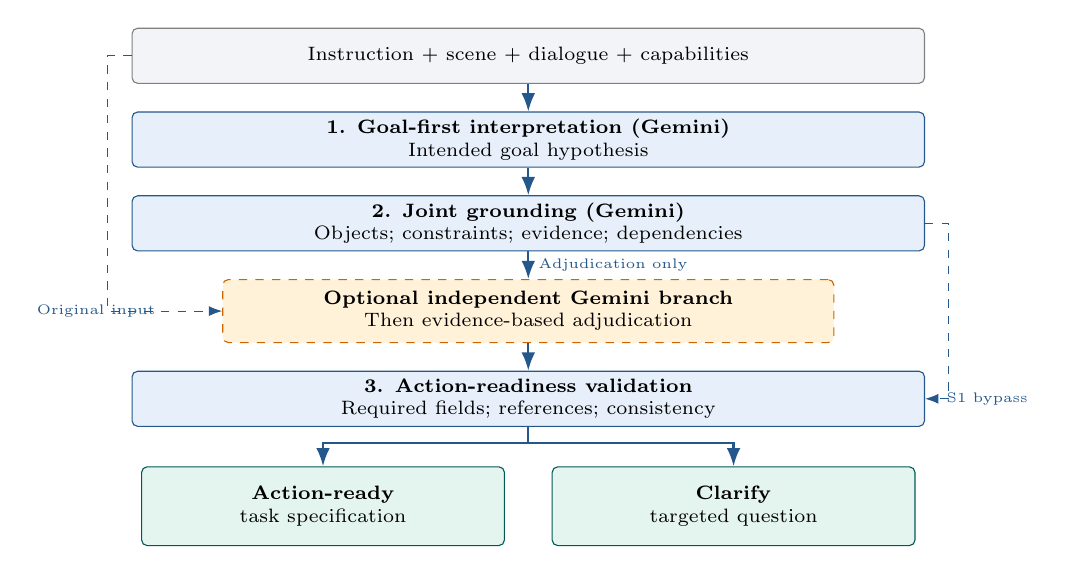
\begin{tikzpicture}[font=\scriptsize,>=Latex,node distance=3.5mm,
 core/.style={draw=deepblue,fill=paleBlue,rounded corners=2pt,minimum width=.83\columnwidth,minimum height=7mm,inner sep=2pt,align=center},
 input/.style={core,fill=paleGray,draw=gray},
 opt/.style={draw=orange!80!black,fill=paleAmber,dashed,rounded corners=2pt,minimum width=.64\columnwidth,minimum height=8mm,align=center,inner sep=2pt},
 resultbox/.style={draw=teal!70!black,fill=paleTeal,rounded corners=2pt,minimum width=.38\columnwidth,minimum height=10mm,align=center,inner sep=2pt}]
\node[input] (i) {Instruction + scene + dialogue + capabilities};
\node[core,below=of i] (g) {\textbf{1. Goal-first interpretation (Gemini)}\\Intended goal hypothesis};
\node[core,below=of g] (t) {\textbf{2. Joint grounding (Gemini)}\\Objects; constraints; evidence; dependencies};
\node[opt,below=of t] (r) {\textbf{Optional independent Gemini branch}\\Then evidence-based adjudication};
\node[core,below=of r] (v) {\textbf{3. Action-readiness validation}\\Required fields; references; consistency};
\node[resultbox,below=5mm of v,xshift=-.215\columnwidth] (ok) {\textbf{Action-ready}\\task specification};
\node[resultbox,below=5mm of v,xshift=.215\columnwidth] (ask) {\textbf{Clarify}\\targeted question};
\draw[->,thick,deepblue] (i)--(g);
\draw[->,thick,deepblue] (g)--(t);
\draw[->,dashed,deepblue] (i.west) -- ++(-3mm,0) |- node[pos=.75,left,font=\tiny]{Original input}(r.west);
\draw[->,thick,deepblue] (t)--node[right,font=\tiny]{Adjudication only}(r);
\draw[->,thick,deepblue] (r)--(v);
\draw[->,thick,deepblue] (v.south)--++(0,-2mm)-|(ok.north);
\draw[->,thick,deepblue] (v.south)--++(0,-2mm)-|(ask.north);
\draw[->,dashed,deepblue] (t.east) -- ++(3mm,0) |- node[pos=.75,right,font=\tiny]{S1 bypass}(v.east);
\end{tikzpicture}
\caption{Proposed interpretation pipeline. S1 bypasses optional review. In S2 the second branch first receives original input only; proposals are shared only for later adjudication. Clarification answers return to grounding and revalidation (feedback omitted).}
\label{fig:pipeline}
\end{figure}

\FloatBarrier
\subsection{Worked example: one choice resolves two fields}
Table~\ref{tab:worked} illustrates the difference between detecting several ambiguities and identifying the particular information needed to complete a task. The example is drawn from case CA-0001 in the co-occurring ambiguity dataset. Its scene identifies two selected medicine trays, assigned respectively to a nurse and a ward clerk. Dialogue establishes that the utterance is a delivery request, and the relevant meal service is at 11:00. Neither fact identifies which tray to deliver. The tray choice is therefore unresolved even though the intended action and time are recoverable.
\begin{table}[!tbp]
\caption{Illustrative grounded interpretation of CA-0001; the user reply is hypothetical, not observed.}
\label{tab:worked}
\centering\footnotesize
\renewcommand{\arraystretch}{1.26}
\begin{tabularx}{\columnwidth}{@{}p{.25\columnwidth}X@{}}
\toprule
\textbf{Element} & \textbf{Interpretation or evidence}\\
\midrule
Utterance & ``Can the selected controlled medicine tray be delivered after a scheduled meal service?''\\
Grounded goal & Deliver a selected controlled medicine tray after the 11:00 meal service.\\
Resolved & Delivery intent; tray type; relevant meal-service time.\\
Missing & Which of the two selected trays is intended?\\
Dependency & Selecting a tray also identifies its assigned recipient.\\
Clarification & ``Which selected controlled medicine tray should I deliver: the nurse's or the ward clerk's?''\\
Conditional output & If the reply is ``the nurse's tray,'' deliver that tray to the nurse after the 11:00 service.\\
\bottomrule
\end{tabularx}
\end{table}
The example illustrates an author-written interpretation of the supplied source, not a stored complete-task gold annotation or measured prediction. The release crosswalk maps former v4 CA-0007 to current CA-0001. The nurse-tray reply is hypothetical and has not been frozen as an evaluation answer. No physical delivery is performed or implied.\todo{Independently verify this illustrative analysis during reference preparation; never use this protected example for prompt tuning or debugging.}
\FloatBarrier

\FloatBarrier
\subsection{Main comparisons and controls}
Table~\ref{tab:systems} summarizes S0 and S1 as the principal systems and S2 as an optional extension. In S2, the second interpretation is generated without seeing the first; adjudication uses input evidence rather than majority voting. Systems receive the same original information and final schema. Five documented run labels and requested API seeds are planned; hosted stochastic decoding is not assumed exactly reproducible. Calls, token budgets, observed tokens, errors and latency must be logged, and S2 inclusion must be decided before evaluated outputs are examined.

\begin{table}[!tbp]
\caption{Planned hosted-model system comparisons}
\label{tab:systems}
\centering
\footnotesize
\begin{tabularx}{\columnwidth}{@{}p{.12\columnwidth}p{.27\columnwidth}X@{}}
\toprule
\textbf{ID} & \textbf{System} & \textbf{Purpose}\\
\midrule
S0 & Direct Gemini & Generate a task or clarification in one pass (baseline).\\
S1 & Structured Gemini & Goal-first interpretation, joint grounding, validation, and clarification (core).\\
S2 (optional) & S1 + Gemini review & Independent second interpretation; optional adjudication of disagreements (extension).\\
\bottomrule
\end{tabularx}
\end{table}

\FloatBarrier
\todo{Pre-register the S0/S1/S2 comparison, matched output schema and reasoning budgets, planned ablations, primary endpoint, and per-case paired uncertainty analysis before evaluating the held-out cases.}
\subsection{Ablations and evaluation}
Within S1, planned ablations independently remove goal-first interpretation, structured intermediate grounding, scene context, dependency checks, and dialogue history. Dialogue eligibility must distinguish merely present history from history relevant to the interpretation. Dependency analysis requires a frozen eligibility annotation identifying linked fields; ambiguity-type labels alone do not establish dependence. Eligible counts are not yet established. The linked-dependency analysis will remain exploratory.

The primary measure is \emph{complete task correctness}: whether all required actions, arguments, and constraints match an independently adjudicated reference in meaning. Secondary measures include per-field grounding accuracy, unsupported-argument rate, missing-critical-field rate, execute/clarify decisions, unnecessary clarification, clarification turns, and inference cost per correctly resolved task. Equivalent task descriptions are judged semantically rather than by literal JSON string matching. Each system is evaluated over five prespecified repeated runs, with identical cases and documented decoding settings; case-level paired comparisons and uncertainty intervals account for variation across cases and runs. Runs are repeated for the ablations where computationally feasible, and any reduced repetition is reported explicitly. Confidence intervals are not calculated by treating repeated outputs from the same case as independent examples. Any evaluation using simulated answers will be clearly separated from evaluation with real user replies.

\todo{Write and test the semantic scoring rubric, confusion-matrix logic, failure-category rules, and independent verification workflow before scoring model outputs.}
\subsection{Failure analysis and scoring procedure}
Every incorrect prediction will be assigned a primary failure category using the same adjudicated reference: wrong intended goal, wrong entity or argument, missing constraint, unsupported inferred detail, unnecessary clarification, or failure to clarify a critical unknown. Secondary tags may be retained when more than one error occurs, but each case contributes once to the primary error count. Reviewers will examine the input evidence and generated structured task, not only the model's explanation. Table~\ref{tab:failure} reserves space for this breakdown in Results.

To score complete task correctness, an evaluator checks the meaning of the full task, including action order and constraints; schema validity alone is insufficient. For a clarification-required case, the initial question is evaluated separately from any task produced after a supplied answer. Disagreements in semantic scoring are resolved using the documented annotation protocol. Results will be reported with the number of eligible cases for each metric.

\subsection{Reproducibility and experimental controls}
Before the first evaluated run, record the requested hosted model ID, returned model-version string, API version, client/runtime versions, prompt and code hashes, decoding settings, requested seeds, context and generation limits, thinking budgets, client location and timestamps. Provider weights, quantization, serving GPU and exact runtime are not controlled by this project; unavailable values must be reported as unavailable. Use the same frozen cases, capability inputs, final schema and scoring procedure across S0 and S1, with S2 optional. Five repeated runs describe stochastic variation, not additional independent cases. Log every call and total latency, including failures and retries. Count reasoning tokens where returned. The primary direct baseline has thinking enabled with a prespecified total budget comparable to S1; non-thinking controls are secondary conditions, not a fourth architecture. Hosted API seeds are requested controls, not guarantees of identical outputs.

The protected cases and all references must not influence prompts, system selection, model choice, or budgets. The published route release is immutable; additional semantic references and the candidate protocol must be completed and frozen before evaluated runs. Annotation provenance and later additions remain auditable.

\todo{Verify live Gemini 2.5 Flash-Lite access and thinking configuration on independent examples; finalize budget fairness, requested seeds, exact prompts, generation limits, API/client versions, warm-up and cost accounting. Freeze these decisions before evaluation. No second model has been selected.}
\subsection{Hosted-model latency and efficiency scope}
The initial efficiency study compares S0 and S1 using the selected Gemini 2.5 Flash-Lite API model; S2 is optional. No second model or smaller hosted checkpoint has been selected, so the earlier six-combination design is not an agreed experiment. Any second-model extension requires a frozen comparison and independent compatibility checks before evaluated outputs are viewed. Measure end-to-end client wall-clock latency including sequential calls, validation and clarification generation; report median and 95th percentile, calls and input/output/reasoning tokens. Record API errors, retry policy, client runtime, request concurrency, warm-up exclusions, collection period and dated pricing. Provider-side GPU memory and hardware are unavailable; TTFT and throughput should be reported only if actually measured. Hosted service variability limits hardware-controlled comparisons. Accuracy--cost claims require verified correctness alongside these measurements.

\FloatBarrier
\section{Results}
\todo{RESULTS NOT RUN. Execute the frozen 100-case evaluation; replace every red TBD table cell and red plot note with measured findings. Do not interpret placeholders as observed evidence.}

\subsection{Action-ready task correctness and routing}
\todo{Compute complete-task correctness, route confusion matrix, unsupported values, uncertainty intervals, and the S0/S1/S2 comparison.}
Table~\ref{tab:mainresults} is reserved for the principal S0/S1 comparison and optional S2 extension. Complete task correctness is the primary outcome; routing correctness and unsupported arguments provide complementary evidence about whether the task was interpreted without guessing. Report denominators and the same metric definitions for each included system. Until full semantic references are available, route-only outputs cannot fill the task-correctness column.
\begin{table}[!tbp]
\caption{Main-system performance (all entries pending).}
\label{tab:mainresults}
\centering\small
\renewcommand{\arraystretch}{1.35}
\begin{tabularx}{\columnwidth}{@{}l>{\centering\arraybackslash}X>{\centering\arraybackslash}X>{\centering\arraybackslash}X@{}}
\toprule
\textbf{System} & \textbf{Task correct (\%)} & \textbf{Route correct (\%)} & \textbf{Unsupported (\%)}\\
\midrule
S0 & \todocell & \todocell & \todocell\\
S1 & \todocell & \todocell & \todocell\\
S2 (optional) & \todocell & \todocell & \todocell\\
\bottomrule
\end{tabularx}
\end{table}
\noindent{\color{todoRed}\textbf{TO DO --- Results interpretation.}}  In the completed report, state which system achieves the highest complete-task accuracy, whether routing and grounding follow the same pattern, and whether observed differences are supported by paired uncertainty intervals. Distinguish an incorrect task from an unnecessary clarification.

\FloatBarrier
\subsection{Stability across repeated runs}
\todo{Run the five prespecified run labels/requested seeds for each included system; replace the empty figure with measured points and means.}
Figure~\ref{fig:runvariation} will display one point for each of five repeated runs per system. The horizontal axis is complete-task correctness; separate rows identify the systems. Add a mean marker and an interval describing variation across runs. This makes instability visible without a large table of individual seeds.
\begin{figure}[!tbp]
\centering
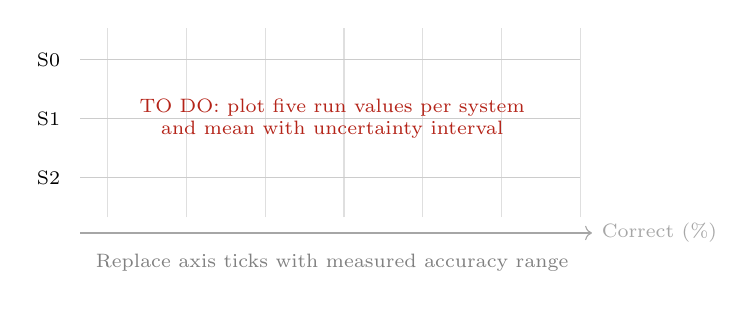
\begin{tikzpicture}[x=1cm,y=1cm,font=\scriptsize]
\draw[->,gray!70] (.65,.35)--(7.15,.35) node[right] {Correct (\%)};
\foreach \x in {1,2,3,4,5,6,7}{\draw[gray!25] (\x,.55)--(\x,2.95);}
\foreach \y/\n in {2.55/S0,1.8/S1,1.05/S2}{\node[anchor=east] at (.52,\y) {\n};\draw[gray!40] (.65,\y)--(7,\y);}
\node[align=center,text=todoRed] at (3.85,1.8) {TO DO: plot five run values per system\\and mean with uncertainty interval};
\node[anchor=north,text=gray] at (3.85,.20) {Replace axis ticks with measured accuracy range};
\end{tikzpicture}
\caption{Temporary plotting template: run-to-run variation in task correctness. No data plotted.}
\label{fig:runvariation}
\end{figure}
\noindent{\color{todoRed}\textbf{TO DO --- Results interpretation.}}  In the completed report, discuss whether rankings remain consistent across repeated runs, the size of the within-system spread, and whether any apparent improvement is smaller than run-to-run variation. Report case-level paired intervals separately from seed variability.

\noindent\textit{Planned reporting detail.} Each plotted point represents one complete evaluation run on the same frozen set of commands. The visual separates variability from decoding and inference from differences between test cases. The accompanying text will report the five-run mean and standard deviation for each system, while paired case-level intervals will be estimated without treating repeated evaluations of one command as independent observations.

\FloatBarrier
\subsection{Correctness versus latency}
\todo{Profile the frozen S0/S1 hosted-model comparison, and S2 only if retained. Report P50/P95 latency and token usage. Define any second-model extension before evaluation rather than assuming six combinations.}
Figure~\ref{fig:tradeoff} reserves space for correctness against measured client end-to-end median latency. Each point represents an actually evaluated system/model configuration; no fixed six-point design is claimed. Include uncertainty, token usage and collection conditions. The 95th-percentile latency is reported in Table~\ref{tab:latency}.
\begin{figure}[!tbp]
\centering
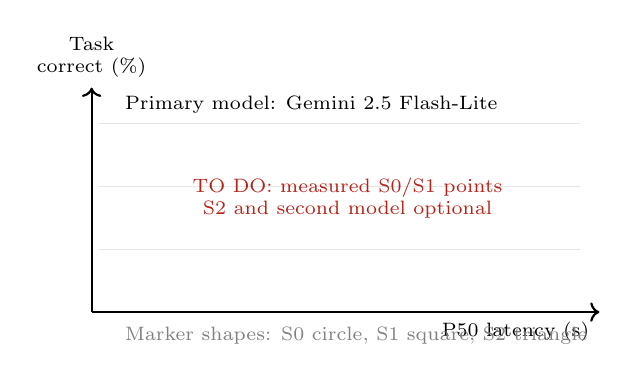
\begin{tikzpicture}[x=1cm,y=1cm,font=\scriptsize]
\draw[->,thick] (.7,.55)--(7.15,.55) node[below left] {P50 latency (s)};
\draw[->,thick] (.7,.55)--(.7,3.4) node[above,align=center] {Task\\correct (\%)};
\draw[gray!20] (.8,1.35)--(6.9,1.35);
\draw[gray!20] (.8,2.15)--(6.9,2.15);
\draw[gray!20] (.8,2.95)--(6.9,2.95);
\node[align=center,text=todoRed] at (3.95,2.0) {TO DO: measured S0/S1 points\\S2 and second model optional};
\node[anchor=west] at (1.0,3.18) {Primary model: Gemini 2.5 Flash-Lite};
\node[anchor=west,text=gray] at (1.0,.25) {Marker shapes: S0 circle, S1 square, S2 triangle};
\end{tikzpicture}
\caption{Temporary plotting template: task correctness versus end-to-end latency. No data plotted.}
\label{fig:tradeoff}
\end{figure}
\begin{table}[!tbp]
\caption{Latency summary (all entries pending).}
\label{tab:latency}
\centering\small
\renewcommand{\arraystretch}{1.32}
\begin{tabularx}{\columnwidth}{@{}lcc>{\centering\arraybackslash}X@{}}
\toprule
\textbf{API model} & \textbf{System} & \textbf{P50 (s)} & \textbf{P95 (s)}\\
\midrule
Flash-Lite & S0/S1 & \todocell & \todocell\\
Optional & S2 / second model & \todocell & \todocell\\
\bottomrule
\end{tabularx}
\end{table}
\noindent{\color{todoRed}\textbf{TO DO --- Results interpretation.}} Interpret measured accuracy and tail latency together; discuss additional calls only for configurations actually evaluated. Record dated API pricing and hosted-service limitations. A second-model or S2 result must remain pending unless that extension was prespecified and completed.

\noindent\textit{Planned reporting detail.} The scatter plot will show whether additional inference produces a measurable correctness benefit relative to its time cost. Median latency measures typical response time, whereas the 95th percentile captures slow responses that may be unsuitable for interactive use. Marker shape identifies the pipeline and colour identifies an actual hosted model, if a second model is later prespecified; the final figure will include actual units and uncertainty intervals.

\FloatBarrier
\subsection{Component and context ablations}
\todo{Run each component/context removal with matched controls; isolate the dependency-linked and dialogue-eligible subsets.}
Table~\ref{tab:ablations} isolates the contribution of intermediate interpretation, grounding, and available context. Differences must be calculated against the corresponding full-S1 result on the same eligible cases, especially for dialogue and linked-dependency subsets.
\begin{table}[!tbp]
\caption{Structured-system ablations (all entries pending).}
\label{tab:ablations}
\centering\small
\renewcommand{\arraystretch}{1.30}
\begin{tabularx}{\columnwidth}{@{}Xcc@{}}
\toprule
\textbf{Configuration} & \textbf{Correct (\%)} & \textbf{$\Delta$ vs. S1 (pp)}\\
\midrule
Full S1 & \todocell & \todocell\\
Without goal-first interpretation & \todocell & \todocell\\
Without structured grounding & \todocell & \todocell\\
Without scene context & \todocell & \todocell\\
Without dependency checking & \todocell & \todocell\\
Without dialogue (eligible cases) & \todocell & \todocell\\
\bottomrule
\end{tabularx}
\end{table}
\noindent{\color{todoRed}\textbf{TO DO --- Results interpretation.}}  In the completed report, describe which removal produces the largest loss, whether context matters more than intermediate structure, and whether dependency checking helps on linked cases rather than only on the full sample. Avoid attributing a causal mechanism to a small numerical difference without supporting case-level evidence.

\noindent\textit{Planned reporting detail.} Every ablation will preserve the evaluation cases and scoring rules of its matched full-system control. Context-removal tests measure sensitivity to available evidence, not performance on an equivalent information task. For the smaller linked-dependency subgroup, results will be reported as exploratory rather than definitive.

\FloatBarrier
\subsection{Error types and qualitative cases}
\todo{Classify errors from scored outputs and write two or three verified case studies grounded in input evidence.}
Table~\ref{tab:failure} will report the dominant causes of incorrect interpretations. This analysis complements overall accuracy by distinguishing errors that might be repaired through more context, better grounding, or targeted clarification. Each category will be illustrated with an anonymized or permitted example, the relevant evidence, and the corrected task interpretation.
\begin{table}[!tbp]
\caption{Failure analysis template (counts and rates pending).}
\label{tab:failure}
\centering\footnotesize
\renewcommand{\arraystretch}{1.32}
\begin{tabularx}{\columnwidth}{@{}Xcc@{}}
\toprule
\textbf{Primary failure type} & \textbf{Count} & \textbf{Rate (\%)}\\
\midrule
Incorrect intended goal & \todocell & \todocell\\
Wrong entity or argument & \todocell & \todocell\\
Missing task constraint & \todocell & \todocell\\
Unsupported inferred detail & \todocell & \todocell\\
Unnecessary clarification & \todocell & \todocell\\
Missing required clarification & \todocell & \todocell\\
\bottomrule
\end{tabularx}
\end{table}
\noindent{\color{todoRed}\textbf{TO DO --- Case interpretation.}} The completed report will identify which error categories dominate for each system and explain two or three representative cases. It will distinguish failures caused by absent input information from failures to use information already present. Any claim about the value of a component will be supported by its corresponding ablation and case-level evidence.

\FloatBarrier
\subsection{Clarification and eventual task completion}
\todo{Run the up-to-five-turn clarification loop with labeled hypothetical answers; graph verified simulated completion separately from real human outcomes.}
Figure~\ref{fig:clarification} will show the cumulative fraction of cases that reach a correct action-ready specification after zero through five clarification turns. Plot S1 and optional S2 separately, and distinguish simulated-answer evaluation from any real human interactions. The denominator must be stated clearly, and a case reaching the turn cap without success remains unresolved.
\begin{figure}[!tbp]
\centering
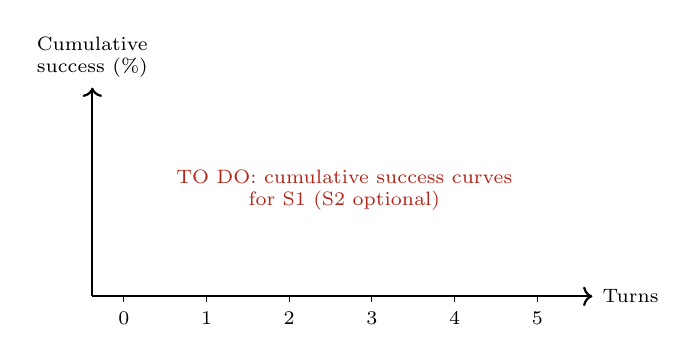
\begin{tikzpicture}[x=1cm,y=1cm,font=\scriptsize]
\draw[->,thick] (.7,.55)--(7.05,.55) node[right] {Turns};
\draw[->,thick] (.7,.55)--(.7,3.2) node[above,align=center] {Cumulative\\success (\%)};
\foreach \i/\x in {0/1.1,1/2.15,2/3.2,3/4.25,4/5.3,5/6.35}{\draw (\x,.55)--(\x,.48) node[below] {\i};}
\node[align=center,text=todoRed] at (3.9,1.9) {TO DO: cumulative success curves\\for S1 (S2 optional)};
\end{tikzpicture}
\caption{Temporary plotting template: eventual task success by clarification turn. No data plotted.}
\label{fig:clarification}
\end{figure}
\noindent{\color{todoRed}\textbf{TO DO --- Results interpretation.}}  In the completed report, explain how often clarification is needed, how quickly it resolves missing information, and whether repeated review reduces unnecessary questions. Report the linked-dependency subgroup separately, with its sample count and uncertainty, rather than claiming a broad effect from a small subgroup.

\noindent\textit{Planned reporting detail.} The zero-turn point records tasks already correct before any question is asked. Later points count only cases that become correct after receiving the corresponding clarification answer. The completed analysis will separate cases that were unnecessarily queried from cases where clarification was necessary but unsuccessful.

\FloatBarrier
\todo{Before Discussion: complete all tables and figures, report sample denominators, repeated-run spread, paired case-level uncertainty, subgroup caveats, and concrete examples of major failures.}
\section{Discussion}
\pending{Reserved for interpretation of verified findings, limitations, and comparison with prior work.}
\section{Conclusion and Future Work}
\pending{Reserved until results and discussion have been completed.}
\section*{Code and Data Availability}
\todo{Release or archive source, environment lockfile, requested/returned API model versions, exact prompts, evaluation scripts, frozen annotation version, and any allowable dataset artifacts; verify reuse licenses.}
The project repository is available at \url{https://github.com/huziibee/Research_Project}. Dataset release conditions, final evaluation splits, and reproducibility artifacts will be specified after the experimental protocol is frozen.
\section*{Acknowledgements}
All praise and thanks are due to Allah, whose mercy, guidance, and blessings made this work possible, and who granted me the strength, patience, and perseverance to complete it. I am deeply grateful to my supervisors, Steven James and Benjamin Rosman, for their guidance, feedback, encouragement, and for continually helping me strengthen the clarity and rigour of this research. I would also like to thank my parents, Mohammed Ebrahim Bangie and Gulshan Bangie, for their unwavering support, patience, encouragement, and sacrifices throughout my studies. Finally, I thank Taruna Naidoo for her support and helpful advice during the preparation of this research report.
\noindent{\color{todoRed}\footnotesize\textbf{TO DO --- References:} Check complete authors, publication venues, years, page/DOI or arXiv identifiers, and live URLs. Cite only code that is actually reused, with its repository/license. Historical annotation-model identities must be reported only from verified package provenance; no unverified model-card claim is added here.}\par\smallskip
\begin{thebibliography}{99}
\bibitem{ambik} A. Ivanova \emph{et al.}, ``AmbiK: Dataset of Ambiguous Tasks in Kitchen Environment.''
\bibitem{tool} Y. Zhang \emph{et al.}, ``Can You Pass That Tool?: Implications of Indirect Speech in Physical Human-Robot Collaboration.''
\bibitem{clara} J. Park \emph{et al.}, ``CLARA: Classifying and Disambiguating User Commands for Reliable Interactive Robotic Agents,'' \emph{IEEE Robotics and Automation Letters}, 2023.
\bibitem{clarifyvc} H. Zhou \emph{et al.}, ``ClarifyVC: Clarifying Ambiguous Commands in Vehicle Control with a Hybrid Data Augmentation Pipeline,'' \emph{ICLR}, 2026.
\bibitem{codraw} B. Madureira and D. Schlangen, ``Instruction Clarification Requests in Multimodal Collaborative Dialogue Games: Tasks, and an Analysis of the CoDraw Dataset.''
\bibitem{sarathy} V. Sarathy, M. Fawn, M. McWilliams, M. Scheutz, and B. Oosterveld, ``On Evaluating LLM Integration into Robotic Architectures.''
\bibitem{mannekote} A. Mannekote \emph{et al.}, ``Making Task-Oriented Dialogue Datasets More Natural by Synthetically Generating Indirect User Requests.''
\bibitem{searle1975} J. R. Searle, ``Indirect Speech Acts, in \emph{Syntax and Semantics}, vol. 3, \emph{Speech Acts}, P. Cole and J. L. Morgan, Eds. New York: Academic Press, 1975, pp. 59--82.
\bibitem{grice1975} H. P. Grice, ``Logic and Conversation, in \emph{Syntax and Semantics}, vol. 3, \emph{Speech Acts}, P. Cole and J. L. Morgan, Eds. New York: Academic Press, 1975, pp. 41--58.



\bibitem{geminimodel} Google, ``Gemini 2.5 Flash-Lite,'' model documentation. \url{https://ai.google.dev/gemini-api/docs/models/gemini-2.5-flash-lite}.
\bibitem{geminithinking} Google, ``Gemini thinking,'' API documentation. \url{https://ai.google.dev/gemini-api/docs/thinking}.
\bibitem{vague} H. Nam \emph{et al.}, ``VAGUE: Visual Contexts Clarify Ambiguous Expressions,'' \emph{Proc. ICCV}, 2025.
\end{thebibliography}
\end{document}
